

\tikzset{every picture/.style={line width=0.75pt}} %set default line width to 0.75pt        
\begin{center}
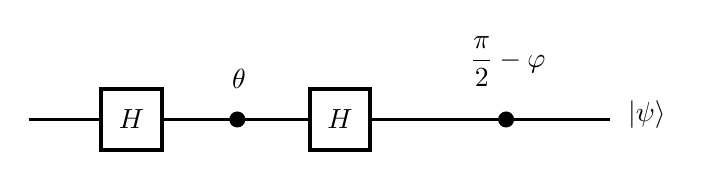
\begin{tikzpicture}[x=0.75pt,y=0.75pt,yscale=-1,xscale=1]
%uncomment if require: \path (0,300); %set diagram left start at 0, and has height of 300

%Straight Lines [id:da06979007227355538] 
\draw    (140.17,140.33) -- (239.17,140.33) ;


%Shape: Rectangle [id:dp49376768989171205] 
\draw  [fill={rgb, 255:red, 255; green, 255; blue, 255 }  ,fill opacity=1 ][line width=1.5]  (175.13,125.5) -- (204.21,125.5) -- (204.21,155.17) -- (175.13,155.17) -- cycle ;
%Straight Lines [id:da007553374828097148] 
\draw    (240.67,140.33) -- (370.17,140.33) ;

\draw [shift={(240.67,140.33)}, rotate = 360] [color={rgb, 255:red, 0; green, 0; blue, 0 }  ][fill={rgb, 255:red, 0; green, 0; blue, 0 }  ][line width=0.75]      (0, 0) circle [x radius= 3.35, y radius= 3.35]   ;
%Shape: Rectangle [id:dp522626456344331] 
\draw  [fill={rgb, 255:red, 255; green, 255; blue, 255 }  ,fill opacity=1 ][line width=1.5]  (275.63,125.5) -- (304.71,125.5) -- (304.71,155.17) -- (275.63,155.17) -- cycle ;
%Straight Lines [id:da11299120546483388] 
\draw    (370.17,140.33) -- (420.42,140.33) ;

\draw [shift={(370.17,140.33)}, rotate = 0] [color={rgb, 255:red, 0; green, 0; blue, 0 }  ][fill={rgb, 255:red, 0; green, 0; blue, 0 }  ][line width=0.75]      (0, 0) circle [x radius= 3.35, y radius= 3.35]   ;

% Text Node
\draw (189.67,140.33) node   {$H$};
% Text Node
\draw (290.17,140.33) node   {$H$};
% Text Node
\draw (438,138) node   {$|\psi \rangle $};
% Text Node
\draw (241.5,121) node   {$\theta $};
% Text Node
\draw (371,112.5) node  [align=left] {$\displaystyle \frac{\pi }{2} -\varphi $};


\end{tikzpicture}
\end{center}